\documentclass[12pt,a4paper]{article}

% ---------------------------------------------------------------
%  PACOTES
% ---------------------------------------------------------------
\usepackage{graphicx}
\usepackage{amsmath}
\usepackage{amssymb}
\usepackage[T1]{fontenc}
\usepackage[utf8]{inputenc}
\usepackage[brazil]{babel}
\usepackage[pagebackref=true,breaklinks=true,colorlinks,bookmarks=false]{hyperref}
\usepackage{geometry}
\geometry{top=2.5cm, bottom=2cm, left=2cm, right=2cm}
\usepackage{setspace}
\usepackage{booktabs}
\usepackage{array}
\usepackage{pgfgantt}
\usepackage{rotating}
\usepackage{indentfirst}
\usepackage[alf]{abntex2cite}
\usepackage{soul}
\usepackage{color}
\usepackage{longtable}
\usepackage{times}
\usepackage{titlesec}
\usepackage{fancyhdr}
\usepackage{tocloft}
\usepackage{float}
\usepackage{caption}
\usepackage{multirow}


% ---------------------------------------------------------------
%  CONFIGURAÇÕES DE ESPAÇAMENTO E FONTE
% ---------------------------------------------------------------
\setstretch{1.5}
\setlength{\parindent}{1.25cm}
\setlength{\parskip}{0pt}
\captionsetup[table]{skip=10pt}

% ---------------------------------------------------------------
%  CONFIGURAÇÃO DOS TÍTULOS DAS SEÇÕES (estilo ABNT)
% ---------------------------------------------------------------
\titleformat{\section}
  {\normalfont\fontsize{12}{14}\bfseries\uppercase}
  {\thesection\quad}
  {0pt}
  {}
\titlespacing*{\section}{0pt}{1.5\baselineskip}{1\baselineskip}

\titleformat{\subsection}
  {\normalfont\fontsize{12}{14}\bfseries}
  {\thesubsection\quad}
  {0pt}
  {}
\titlespacing*{\subsection}{0pt}{1\baselineskip}{0.3\baselineskip}

\titleformat{\subsubsection}
  {\normalfont\fontsize{12}{14}\bfseries}
  {\thesubsubsection\quad}
  {0pt}
  {}
\titlespacing*{\subsubsection}{0pt}{1\baselineskip}{0.3\baselineskip}

% ---------------------------------------------------------------
%  CONFIGURAÇÃO DO CABEÇALHO/RODAPÉ
% ---------------------------------------------------------------
\fancypagestyle{pretextual}{
  \fancyhf{}
  \renewcommand{\headrulewidth}{0pt}
}

\fancypagestyle{plain}{
  \fancyhf{}
  \fancyhead[R]{\thepage}
  \renewcommand{\headrulewidth}{0.5pt}
}

\renewcommand{\sectionmark}[1]{\markboth{\thesection\ \ \MakeUppercase{#1}}{}}

\pagestyle{fancy}
\fancyhf{}
\fancyhead[L]{\nouppercase{\leftmark}}
\fancyhead[R]{\thepage}
\renewcommand{\headrulewidth}{0.5pt}

% ---------------------------------------------------------------
%  CONFIGURAÇÃO DO SUMÁRIO E LISTAS
% ---------------------------------------------------------------
\renewcommand{\cftfigpresnum}{Figura~}
\setlength{\cftfignumwidth}{3.2cm}

\renewcommand{\cfttabpresnum}{Tabela~}
\setlength{\cfttabnumwidth}{3.2cm}

\renewcommand{\cftsecfont}{\bfseries}
\renewcommand{\cftsecpagefont}{\bfseries}
\renewcommand{\cftsubsecfont}{\normalfont}

\renewcommand{\cftsecdotsep}{\cftdotsep}

% ---------------------------------------------------------------
%  METADATA
% ---------------------------------------------------------------
\hypersetup{
  pdftitle={Otimização de Portfólio: Pipeline Completo de Metamodelagem e Otimização de Portfólio de Ações},
  pdfauthor={Mateus Matzkin Gurza},
  colorlinks=true,
  linkcolor=black,
  citecolor=black,
  urlcolor=black
}

% ---------------------------------------------------------------
%  INÍCIO DO DOCUMENTO
% ---------------------------------------------------------------
\begin{document}
\pagenumbering{arabic}

% ---------------------------------------------------------------
%  CAPA
% ---------------------------------------------------------------
\begin{titlepage}
\thispagestyle{pretextual}
\begin{center}


\includegraphics[height=3cm]{images/Logo_Escola-Politecnica-Minerva-com-fundo.png}
\hfill

\includegraphics[height=2cm]{images/USP-1320x743.jpg}

\vspace{3cm}

{\fontsize{12}{14}\selectfont ESCOLA POLITÉCNICA DA USP}

\vspace{1cm}

{\fontsize{12}{14}\selectfont MATEUS MATZKIN GURZA}

\vspace{4cm}

{\fontsize{12}{14}\bfseries\MakeUppercase{Otimização de Portfólio: Pipeline Completo de Metamodelagem e Otimização de Portfólio de Ações}}

\vfill

{\fontsize{12}{14}\selectfont São Paulo}\\[4pt]
{\fontsize{12}{14}\selectfont \the\year}

\end{center}
\end{titlepage}

% ---------------------------------------------------------------
%  FOLHA DE ROSTO
% ---------------------------------------------------------------
\newpage
\thispagestyle{pretextual}
\begin{center}

{\fontsize{12}{14}\selectfont ESCOLA POLITÉCNICA DA USP}

\vspace{1cm}

{\fontsize{12}{14}\selectfont MATEUS MATZKIN GURZA \quad VINICIUS BARILE LORA FRANCO}

\vspace{4cm}

{\fontsize{12}{14}\bfseries\MakeUppercase{Otimização de Portfólio: Pipeline Completo de Metamodelagem e Otimização de Portfólio de Ações}}

\end{center}

\vspace{2.5cm}

\begin{flushright}
\begin{minipage}{8cm}
{\fontsize{12}{14}\selectfont
Trabalho apresentado à disciplina PRO6006 - Métodos de Otimização Não Linear com aplicações em machine learning, do programa de pós-graduação, como requisito de avaliação, demonstrando a compreensão do curso e a aplicação de processos de otimização não linear a um caso prático.}

\vspace{1cm}

{\fontsize{12}{14}\selectfont Professora: Profa. Dra. Celma O. Ribeiro}
\end{minipage}
\end{flushright}

\vfill

\begin{center}
{\fontsize{12}{14}\selectfont São Paulo}\\[4pt]
{\fontsize{12}{14}\selectfont \the\year}
\end{center}

% ---------------------------------------------------------------
%  RESUMO
% ---------------------------------------------------------------
\newpage
\thispagestyle{pretextual}
\begin{center}
{\fontsize{12}{14}\bfseries RESUMO}
\end{center}
\vspace{1em}

\noindent
A seleção de um portfólio de investimento busca, para um dado conjunto de ativos, a combinação de alocações que ofereça o melhor equilíbrio entre retorno esperado e risco para um determinado investidor. A formulação clássica, baseada no retorno médio, na variância de cada ativo e na correlação entre eles, foi o pontapé inicial para a construção de um campo robusto de estudos acerca dos diferentes métodos de realizar essa seleção. Nesse contexto o interesse deste trabalho está no processo de otimização que leva à carteira recomendada. O projeto propõe um pipeline completo de seleção, que vai da coleta de dados de preços de ações à obtenção de uma carteira ótima. A carteira é escolhida pela otimização de uma função objetivo, neste caso, a minimização do Valor-em-Risco Condicional (CVaR), e comparada aos resultados obtidos pela formulação clássica de Média-Variância. O processo de otimização em si é realizado por meio de otimização bayesiana apoiada em um modelo substituto, aplicada a um conjunto pré-definido de ações da bolsa americana obtido pela Yahoo Finance. O produto esperado é o pipeline funcional e a análise do processo de otimização projetado.

\vspace{1em}
\noindent
\textbf{Palavras-chave:} otimização de portfólio; otimização não linear; otimização bayesiana; modelo substituto; índice de Sharpe.

\newpage
\thispagestyle{pretextual}
\tableofcontents

% ---------------------------------------------------------------
%  INÍCIO DO TEXTO
% ---------------------------------------------------------------
\newpage
\pagestyle{fancy}
\thispagestyle{plain}

% ===============================================================
%  1. INTRODUÇÃO
% ===============================================================
\section{Introdução}

A seleção da composição de um portfólio de investimentos tem por objetivo, para um investidor que se comporte de forma racional, encontrar uma combinação de ativos que ofereça o maior retorno possível para um dado nível de risco, ou o menor risco possível para um dado nível de retorno \cite{markowitz1952portfolio}. A hipótese de comportamento é a de que, ao ter que escolher entre duas carteiras com o mesmo retorno esperado, o investidor escolhe sempre a de menor risco \cite{markowitz1952portfolio}.

A teoria moderna de carteiras, formulada por \citeonline{markowitz1952portfolio}, propõe que a decisão de investimento seja tomada com base na análise conjunta de retorno esperado e risco. Cada combinação desses dois parâmetros corresponde a um nível de utilidade para o investidor. Como há um \textit{tradeoff} entre retorno e risco com relação à utilidade, é possível definir curvas ao longo das quais a utilidade permanece constante, chamadas curvas de indiferença ,ou, em outras palavras, configurações distintas de carteira que produzem o mesmo grau de satisfação. Entre duas curvas, o investidor prefere aquela que, para o mesmo nível de risco, oferece retorno mais alto.

O conjunto de todas as carteiras possíveis, correspondente a todas as distribuições possíveis do capital entre as ações disponíveis, forma uma região no espaço definido pelos riscos e retornos possíveis. Os portfólios para os quais não existe alternativa melhor, ou seja, nenhuma outra com mais retorno para o mesmo risco nem com menos risco para o mesmo retorno, formam a "fronteira eficiente" \cite{markowitz1952portfolio}. O portfólio eficiente é, portanto, aquele que reside na borda superior dessa região. O ponto específico da fronteira escolhido pelo investidor depende de sua tolerância ao risco, e esse ponto é o portfólio ótimo \cite{markowitz1952portfolio}.

Para entender o processo de seleção de um portfólio, então, é preciso definir três entidades: o retorno de um ativo e de uma carteira, o risco associado, medido pela variância, e a correlação entre os ativos (covariância). É justamente a covariância que, na teoria clássica de seleção de portfólios, guia o processo completo de diversificação de ações no portfólio e explica por que combinar ativos pode reduzir o risco sem sacrificar o retorno médio. Esses conceitos são mais desenvolvidos na Seção~\ref{sec:fundamentacao}.

As ideias de Markowitz (1952) foram decisivas no campo, mas apresentam limitações práticas que, posteriormente, motivaram esforços de aprimoramento nos métodos de seleção de portfólio. A limitação mais relevante para a proposta de projeto aqui documentada é a da sensibilidade extrema da carteira ótima à estimativa do retorno esperado, um parâmetro difícil de estimar. \citeonline{black1992global} documentam que a otimização de "média-variância" proposta por Markowitz (1952), que usa uma aproximação desse retorno esperado estimado por meio da média de dados históricos, tende a produzir carteiras com posições extremas e pouco intuitivas, muito sensíveis a pequenas variações nas entradas. Isso ocorre, segundo os autores, por tratar as estimativas como se fossem certezas.

Trabalhos mais recentes buscaram tratar com maior prioridade essa incerteza envolvida no problema. A análise bayesiana de média-variância de \citeonline{bauder2021bayesian} e a abordagem geral de \citeonline{bade2009general} substituem a suposição de parâmetros conhecidos por uma distribuição de possibilidades, de modo que a definição da carteira já envolve a estocasticidade e a imperfeição dos dados. Com a complexidade crescente no processo de definição de parâmetros, a literatura de otimização passou a tratar a busca pela carteira ótima como um problema de solucionar o alto custo computacional da simulação de cenários. \citeonline{millar2025bayesian} e \citeonline{you2025improving} aplicam otimização bayesiana com modelos substitutos a esse contexto, e \citeonline{moran2026balancing} detalham o compromisso entre exploração e explotação que governa esse tipo de busca.

Este projeto se posiciona na discussão de como selecionar eficientemente um portfólio ótimo, mas com o objetivo de atuar como um \textit{pipeline} integrador. Cada uma das referências consultadas resolve uma parte do problema: coleta de dados, estimativa de parâmetros, escolha de métrica, busca da carteira ótima ou validação. Busca-se aqui, complementando esse compilado de referências já existentes no campo, construir o fluxo inteiro da captação de dados à seleção do portfólio em um único trabalho. A proposta é, assim, construir esse \textit{pipeline} de ponta a ponta, de forma simples, concisa, acessível e reprodutível, aplicando otimização não linear a um caso real. As decisões de escopo, detalhadas na Seção~\ref{sec:plano}, foram tomadas levando em conta essa proposta.

\subsection{Objetivo}

O objetivo principal do projeto é aplicar e compreender técnicas de otimização não linear no contexto da seleção de carteira, construindo e validando um \textit{pipeline} completo que vai da coleta de dados de preços à recomendação de uma carteira. A otimização é conduzida por otimização bayesiana apoiada em um \textit{surrogate model}, e a função objetivo otimizada é o Valor-em-Risco Condicional (CVaR) da carteira.

O produto esperado é o \textit{pipeline} funcional e a análise de ao menos uma carteira ótima obtida por ele, para um conjunto pré-definido de ações da bolsa americana, acessível pelo \textit{Yahoo Finance}. O critério de validação é o desempenho da carteira fora da amostra, calculado ao otimizar a relação de retorno e risco em um período e testar a carteira resultante em um período seguinte, cujo resultado já é conhecido. Esse critério é então comparado ao desempenho do método de Média-Variância (controle), elaborado por Markowitz, cujo desempenho e funcionamento já é bem conhecido no campo.

% ===============================================================
%  2. REVISÃO BIBLIOGRÁFICA
% ===============================================================
\section{Revisão Bibliográfica}
\label{sec:fundamentacao}
Esta seção reúne a revisão bibliográfica que dá suporte ao projeto. Mais do que um levantamento de referências, ela apresenta e organiza os conceitos que formam a fundamentação teórica do trabalho, passando tanto pelas noções de finanças necessárias para entender o que é uma carteira e como se mede seu desempenho, quanto pelas definições matemáticas e pelos métodos de otimização que sustentam o processo de seleção. Os conceitos aqui reunidos são retomados de forma aplicada no plano de projeto da Seção~\ref{sec:plano}.

\subsection{Ações e Retornos}

Uma ação pode ser definida como uma pequena parte do valor total de uma empresa. Assim sendo, é considerada um ativo intangível, por não possuir utilidade física direta, e de renda variável, por não garantir rentabilidade, ou seja, não garantir um retorno. É dessa não garantia de um retorno que deriva o risco de uma ação. O ganho ou perda percentual de um ativo $i$ ao longo de um período, seu retorno, é a variação relativa do preço \cite{markowitz1952portfolio}, conforme indicado na equação \ref{eq retorno}. É importante ressaltar que ações podem passar por processos mais complexos do que apenas a valorização ou desvalorização, como por exemplo o retorno de dividendos, incorporado também na fórmula mas não explicado a fundo neste documento por não ser o foco do projeto.
\begin{equation}
\label{eq retorno}
R_{i,t} = \frac{P_{i,t} + D_{i,t} - P_{i,t-1}}{P_{i,t-1}},
\end{equation}
A equação define um retorno $R_{i,t}$, onde $P_{i,t}$ é o preço do ativo no instante $t$ e $D_{i,t}$ o dividendo pago no período. Como dito anteriormente, ações podem passar por processos que não só a passagem de tempo, como também o desdobramento ou agrupamento de ações, onde a participação de cada acionista permanece a mesma mas o número de ações cresce e seu valor é então diluído. Esse tipo de caso poderia causar uma análise enganosa da variação do preço de uma ação e, por conta disso, ao longo do projeto trabalha-se com preços ajustados, que já incorporam dividendos e desdobramentos, o que permite escrever o retorno diretamente a partir da razão de preços ajustados. 

Outra forma de representar essa razão, é por meio da utilização de Log-Retornos, conforme a equação \ref{eq retorno log}. Está é uma prática comum no campo por possibilitar tratar o caráter multiplicativo dos retornos de forma aditiva \cite{barrosa2015aplicacao}.
\begin{equation}
\label{eq retorno log}
R_{log; i,t} = \log\bigg[\frac{P_{i,t} + D_{i,t} - P_{i,t-1}}{P_{i,t-1}}\bigg],
\end{equation}

Uma carteira ou portfólio é um conjunto de $n$ ativos, cada um com um peso $w_i$ que representa a fração do capital total alocada naquele ativo. Mais especificamente no trabalho aqui proposto, os ativos a compor a carteira serão exclusivamente ações. A soma dos pesos $w_i$ resulta em $100\%$, pois representam a totalidade do capital investido. Assim, o retorno da carteira é a média dos retornos dos ativos ponderada pelos seus respectivos pesos \cite{fabozzi2008portfolio}:

\begin{equation}
\sum_{i=1}^{n} w_i = 1, \qquad    R_p = \sum_{i=1}^{n} w_i R_i = \mathbf{w}^\top \mathbf{R},
\end{equation}

onde $\mathbf{w} = (w_1, \dots, w_n)^\top$ e $\mathbf{R} = (R_1, \dots, R_n)^\top$. 


\subsection{Retorno esperado}

O retorno esperado $\boldsymbol{\mu}$ é a melhor estimativa de quanto cada ativo renderá no futuro, sendo essencial para a tomada de decisão acerca da composição de uma carteira. Veja na equação \ref{eq ret esperado}
\begin{equation}
\label{eq ret esperado}
\mathbb{E}[R_p] = \mathbf{w}^\top \boldsymbol{\mu}, \qquad \boldsymbol{\mu} = \mathbb{E}[\mathbf{R}].
\end{equation}

A forma mais direta de estimar $\boldsymbol{\mu}$ é usando a média dos retornos passados \cite{markowitz1952portfolio}. No entanto, estimar retornos futuros a partir da média de retornos passado é particularmente instável \cite{fisher1935design}. Este é o ponto mais delicado de toda a construção. A estimativa do retorno esperado a partir do histórico é imprecisa, e sua imprecisão decresce lentamente com o tamanho da amostra, ao passo que a estimativa da volatilidade e covariância, discutida a seguir, converge de forma mais rápida. Em outras palavras, com uma amostra limitada é fácil aproximar o risco de um ativo, mas difícil estimar o seu retorno futuro \cite{fisher1935design}. 

Como a carteira ótima de média-variância \cite{markowitz1952portfolio} é muito sensível a $\boldsymbol{\mu}$, carteiras calculadas com médias históricas cruas costumam ser instáveis, concentradas em poucos ativos e decepcionantes fora da amostra usada para estimar a média de retorno. Essa fragilidade é discutida ao longo de todo o projeto e motiva a escolha de uma função objetivo simples e consolidada, discutida na Subseção~\ref{sub:objetivos}.

\subsection{Variância, Volatilidade e Risco das Ações}

O risco de um ativo mede quão incerto é seu retorno. Essa incerteza tem uma ligação íntima com a ideia de renda variável e, portanto, se conecta diretamente ao mercado de ações. Cada ação tem seu respectivo comportamento ao longo do tempo, ações que se comportam de forma oscilatória exagerada e pouco previsível são ações de maior risco. Considerando isso, na formulação de Markowitz (1952), o risco é quantificado pela variância dos retornos, que mede o espalhamento do preço da ação em torno da sua média ao longo do tempo:
\begin{equation}
\sigma_i^2 = \mathbb{E}\big[(R_i - \mu_i)^2\big].
\end{equation}
A raiz quadrada da variância é o desvio padrão $\sigma_i$, chamado de volatilidade no mercado financeiro. Variância alta significa retorno imprevisível, e é essa imprevisibilidade que pode ser traduzida como risco. Resumindo, ações mais voláteis são mais arriscadas.

\subsection{Covariância, Diversificação e Risco da Carteira}

A covariância é um conceito central da teoria de portfólios. Ela mede se dois ativos tendem a se mover juntos, em direções opostas ou de forma independente. De forma geral, ela calcula se o desvio do retorno $R_i$ de uma ação $A$ com relação à sua média  $\mu_i$ e o desvio do retorno $R_j$ de uma ação $B$ com relação à sua média $\mu_j$ ocorrem em sintonia (resultado positivo) ou em oposição (resultado negativo) \cite{markowitz1952portfolio}.
\begin{equation}
\sigma_{ij} = \mathrm{Cov}(R_i, R_j) = \mathbb{E}\big[(R_i - \mu_i)(R_j - \mu_j)\big].
\end{equation}

Seguindo uma lógica similar podemos definir a correlação entre as ações $A$ e $B$ da seguinte maneira: $\rho_{ij} = \sigma_{ij} / (\sigma_i \sigma_j)$, equação essa que normaliza a covariância dividindo-a pelas variâncias individuais das ações, tal que o resultado esteja sempre entre $-1$ e $+1$. Quanto mais próxima de $+1$ for a correlação, mais as duas ações variam em sintonia; Quanto mais próxima de $-1$ mais oposto é o comportamento de uma em relação à outra; e, no meio do caminho, o resultado de correlação $0$ indica que as duas ações podem ser consideradas totalmente independentes uma da outra \cite{markowitz1952portfolio}. 

Reunindo todas as covariâncias na matriz $\boldsymbol{\Sigma}$, de elemento genérico $\sigma_{ij}$, a variância da carteira pode ser definida pelo termo à direita na equação~\eqref{eq:varport}
\begin{equation}
\sigma_p^2 = \sum_{i=1}^{n}\sum_{j=1}^{n} w_i w_j \sigma_{ij} = \mathbf{w}^\top \boldsymbol{\Sigma} \mathbf{w}.
\label{eq:varport}
\end{equation}

A Equação~\eqref{eq:varport} justifica matematicamente a diversificação e é a razão pela qual toda a teoria de portfólios foi elaborada. O risco da carteira não é a média dos riscos individuais: ele depende crucialmente dos termos cruzados $w_i w_j \sigma_{ij}$ referentes a duas diferentes ações e a a forma como variam uma em relação à outra. Quando dois ativos têm covariância baixa ou negativa, suas oscilações se cancelam parcialmente, e a variância do conjunto fica abaixo da média ponderada das variâncias individuais. É possível, assim, montar uma carteira menos arriscada que qualquer um de seus ativos isolados, sem sacrificar o retorno médio. A consequência prática direta para este projeto é que o objetivo a ser otimizado deve ser sempre definido no nível da carteira inteira, pois é a interação entre ativos, capturada por $\boldsymbol{\Sigma}$, que determina a qualidade do conjunto \cite{markowitz1952portfolio}.

\subsection{Abordagem média-variância e a fronteira eficiente}
\label{sec: med var}

Reunindo os elementos anteriores, a seleção de portfólio proposta por Markowitz (1952) pode ser escrita como um problema de otimização. Veja a seguir uma formulação comum que minimiza o risco sujeito a um retorno alvo $\mu^\ast$:
\begin{equation}
\min_{\mathbf{w}} \ \mathbf{w}^\top \boldsymbol{\Sigma} \mathbf{w}
\quad \text{sujeito a} \quad
\mathbf{w}^\top \boldsymbol{\mu} = \mu^\ast, \quad \mathbf{w}^\top \mathbf{1} = 1.
\label{eq:markowitz}
\end{equation}
Entende-se da formulação de Markowitz (média-variância), que para evitar altos riscos na carteira devemos reduzir a volatilidade conjunta dela, e que isso pode ser feito minimizando a covariância ponderada pelos pesos cruzados entre os ativos nela. Considera-se também que essa minimização esta sujeita a um objetivo de retorno, e que variando esse alvo $\mu^\ast$, o conjunto de soluções descreve uma fronteira contendo a carteira menos arriscada para o retorno desejado, essa curva é chamada de fronteira eficiente do plano de risco-retorno definido. Em outras palavras, cada ponto da fronteira é a carteira de menor variância para aquele nível de retorno. A escolha do portfólio final depende da tolerância ao risco do investidor.

\subsection{Funções objetivo e a estimativa do retorno esperado}
\label{sub:objetivos}

A formulação de média-variância, apresentada anteriormente, define o compromisso entre risco e retorno, mas deixa duas perguntas em aberto. A primeira é como transformar esse compromisso em um único número a ser otimizado, já que risco e retorno por si só não indicam qual carteira escolher sem antes fixar um dos dois como restrição. A segunda, mais grave, decorre de um problema já mencionado na Subseção~\ref{sec:fundamentacao}: a equação~\eqref{eq:markowitz} trata $\boldsymbol{\mu}$ como se fosse um valor certo e conhecido, quando na prática é apenas uma estimativa ruidosa. Como os pesos ótimos resultam de uma otimização em que o retorno entra de forma direta e a estimativa de $\boldsymbol{\mu}$ pode variar bastante de uma amostra para outra, pequenas mudanças na estimativa do retorno esperado podem levar a mudanças bruscas na composição da carteira ótima, sobretudo quando os ativos são muito correlacionados entre si. Esse é o problema de fundo que gerou grande parte dos desenvolvimentos posteriores a Markowitz.

As três extensões apresentadas nesta subseção respondem, cada uma à sua maneira, a essas duas perguntas. O índice de Sharpe e o CVaR são duas formas diferentes de resumir risco e retorno em um único objetivo, cada uma adequada a um tipo de comportamento dos dados. O CAPM, por sua vez, ataca diretamente o problema da estimativa de $\boldsymbol{\mu}$, ancorando o retorno esperado em um ponto de equilíbrio de mercado em vez de depender apenas da média histórica de cada ativo. Tratamentos mais elaborados dessa incerteza, de natureza bayesiana, existem na literatura e são retomados nas conclusões desta seção como estado da arte, mas ficam fora do escopo deste trabalho.

\subsubsection{Índice de Sharpe}
\label{sec: sharpe}

Uma forma direta de resumir risco e retorno em um único número é o índice de Sharpe, que mede quanto uma carteira é rentável acima de um ativo sem risco, quantificando quanto se ganha a mais que esse ativo por unidade de risco assumido \cite{sharpe1994sharpe}:
\begin{equation}
S_p = \frac{\mathbf{w}^\top \boldsymbol{\mu} - r_f}{\sqrt{\mathbf{w}^\top \boldsymbol{\Sigma} \mathbf{w}}},
\label{eq:sharpe}
\end{equation}
em que $r_f$ é o retorno do ativo sem risco, tipicamente um título público de curto prazo. Um Sharpe alto indica muito retorno por pouco risco. A Equação~\eqref{eq:sharpe} usa a variância completa da carteira, incorporando a covariância pelo termo $\mathbf{w}^\top \boldsymbol{\Sigma} \mathbf{w}$.

O índice de Sharpe carrega, no entanto, uma suposição implícita: a de que a distribuição dos retornos da carteira é aproximadamente normal, ou seja, que ela fica inteiramente descrita por apenas dois números, a média e o desvio padrão. Por conta dessa suposição, dois desvios de mesma magnitude, um para cima e outro para baixo, são igualmente prováveis e igualmente penalizados pela variância. Essa suposição é conveniente, mas nem sempre corresponde ao comportamento real dos retornos de ações, e nem à penalização que desejamos aplicar ao problema, dado que um desvio para cima e relação ao retorno médio é positivo e um para baixo é negativo, como discutido a seguir \cite{fabozzi2008portfolio}.

\subsubsection{CVaR}

Os retornos de ativos financeiros costumam apresentar dois comportamentos que fogem da distribuição normal, e por isso estão desalinhados com as suposições do índice de Sharpe. O primeiro é a presença de caudas pesadas: quedas e altas muito grandes acontecem com uma frequência maior do que uma distribuição normal preveria. Na prática, isso significa que eventos que a normal trataria como praticamente impossíveis, como uma queda de vários desvios padrão em um único dia, ocorrem no mercado real com uma frequência bem maior do que essa suposição sugere. O segundo é a assimetria: os movimentos de queda tendem a ser mais abruptos e mais frequentes do que movimentos de alta de magnitude equivalente. A consequência prática dessas duas características é que se as desconsiderarmos iremos penalizar de forma incoerente os riscos observados por meio da série temporal do preço da carteira de ações \cite{fabozzi2008portfolio, rockafellar2000optimization}. 

Sendo assim, este problema aparece no índice de Sharpe ao passo que a variância, usada nele, penaliza da mesma forma um desvio para cima e um desvio para baixo, quando na realidade o investidor só se importa com o desvio para baixo. Duas carteiras podem ter o mesmo índice de Sharpe e, ainda assim, exposições muito diferentes a perdas grandes, se uma delas tiver retornos com cauda mais pesada do que a outra. Tendo em vista esse problema, novas funções objetivo foram definidas para evitar essa premissa de simetria indesejável, como por exemplo o VaR\footnote{O VaR, precursor e base fundamental para a criação do CVaR, quantifica a perda máxima a um determinado nível de confiança $\alpha$. Foi substituído pelo CVaR por ignorar a magnitude das perdas associadas ao peso da cauda (risco de cauda) e por não ter a propriedade de subaditividade \cite{barrosa2015aplicacao}.} e o CVaR. Ambas as funções estão exemplificadas de forma ilustrativa na figura \ref{fig:cvar_var}, onde VaR e CVaR são identificados justamente em um caso onde as premissas de normalidade (curva pontilhada) e simetria, causariam problemas para outras funções objetivo. 

\begin{figure}[htbp]
    \centering
    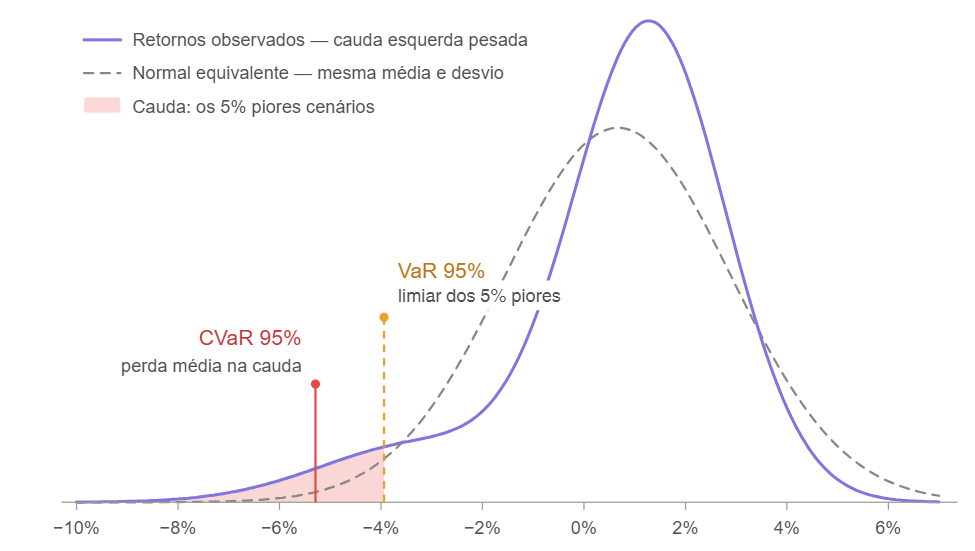
\includegraphics[width=0.8\textwidth]{images/cvar_var.png}
    \caption{Esquema lúdico ilustrativo de VaR e CVaR a 95\% em uma distribuição com cauda esquerda pesada, comparada à normal de mesma média e desvio-padrão. Fonte: elaboração própria, dados simulados.}
    \label{fig:cvar_var}
\end{figure}

O Valor-em-Risco Condicional, ou CVaR, é uma medida de risco pensada para focar exatamente no ponto cego do índice Sharpe. Em vez de resumir toda a distribuição em um desvio padrão, o CVaR olha apenas para a fatia mais extrema das perdas e calcula a perda média dentro dessa fatia \cite{rockafellar2000optimization}. O tamanho dessa fatia é definido por um nível de confiança $\alpha$: por exemplo, com $\alpha$ igual a $95\%$, olha-se apenas para os $5\%$ piores cenários de perda e calcula-se a perda média entre eles. Formalmente, sendo $L$ a perda da carteira e $\mathrm{VaR}_\alpha$ o quantil de nível $\alpha$ da distribuição de perdas, que separa os piores cenários do restante,
\begin{equation}
\mathrm{CVaR}_\alpha = \mathbb{E}\big[\, L \mid L \geq \mathrm{VaR}_\alpha \,\big].
\end{equation}
Quanto maior o $\alpha$ escolhido, mais a medida se concentra nos cenários mais raros e mais catastróficos, o que a torna mais sensível justamente às caudas pesadas que o índice de Sharpe ignora \cite{rockafellar2000optimization}.

Assim, o problema de otimização proposto na utilização do CVaR é o equacionado a seguir:

\begin{equation}
\min_{\mathbf{w}} \ \mathrm{CVaR}_\alpha(\mathbf{w})
\quad \text{sujeito a} \quad
\mathbf{w}^\top \boldsymbol{\mu} \geq \mu_{\min}, \quad
\mathbf{w}^\top \mathbf{1} = 1, \quad
\mathbf{w} \geq 0.
\label{eq:cvar_opt}
\end{equation}

 Um ponto relevante desse trabalho é que o CVaR é uma função difícil de otimizar. Essa dificuldade tem origem em dois principais fatores: primeiro, as características  superfície resultante da função sobre o domínio de composições $\mathbf{w} \in \mathbb{R}^n$; segundo, a quantidade de cenários que é necessário simular para cobrir um domínio completo de $n$ dimensões, correspondentes ao número de ativos distintos na carteira.  Existem diferentes formas de calcular o VaR e consequentemente o CVaR resultante. A escolha de qual método usar depende de qual distribuição se assume para os retornos, sendo que essa decisão afeta também a qualidade e precisão do modelo. 
 
 No caso da distribuição normal, utiliza-se o método paramétrico para o qual se assume, conforme a teoria clássica de estatística, $\mathrm{VaR_\alpha} = \mu-z_{\alpha}\sigma$ \cite{barrosa2015aplicacao}. No entanto, embora mais barata, tal formulação desconsidera o risco de cauda, assim como outras formulações que exigem assumir uma distribuição gaussiana para estimar retornos futuros. Outra opção é utilizar o método não paramétrico, que, embora mais caro computacionalmente, é capaz de lidar com o risco de cauda. Nele se aplica um estimador do valor do percentil para a confiança $\alpha$ definida, sendo esse estimador representado por $M_{[\alpha T:T]}(R)$ tal que o VaR é definido pela seguinte sequência de passos, conforme a estatística de ordem \cite{barrosa2015aplicacao}:
 \begin{enumerate}
     \item Toma-se uma amostra histórica de tamanho $T$ de retornos $R_p$, com periodicidade $p$ desejada, de uma carteira com uma composição $\mathbf{w}$ fixa para a qual se está calculando o $\mathrm{VaR}_\alpha(\mathbf{w})$ com $\alpha \in [0,1]$;
     \item Ordena-se essa amostra de tamanho $T$ do menor para o maior retorno, assim a assimetria continua sendo capturada;
     \item O VaR é o valor na posição $M_{[\alpha T:T]}(R_p)$, ou seja, o $\alpha T$-ésimo valor de retorno para um periodo $p$ em ordem crescente, representando um percentil empírico da amostra ordenada;
     \item O passo extra necessário para calcular o CVaR a partir desse método é, então, realizar a média dos valores da amostra que ficam além desse VaR calculado.
 \end{enumerate}
 Assim, no método não paramétrico com estimador $M_{[\alpha T:T]}(R_p)$ estimamos o retorno $R_p$ correspondente ao $\mathrm{VaR}_\alpha(\mathbf{w})$, cujo valor representa a pior perda esperada para um período $p$ pelo qual deixamos o capital investido numa carteira de composição $\mathbf{w}$ com uma confiança $\alpha$ \cite{barrosa2015aplicacao}. Com esse valor somos capazes de calcular o CVaR para a mesma amostra, que pode ser entendido como o valor esperado da perda em um periodo $p$ quando o limite do VaR para uma dada confiança é ultrapassado, sendo que $\mid\mathrm{CVaR}\mid > \mid\mathrm{VaR}\mid$ \cite{barrosa2015aplicacao}. 

 O método "puro" de calcular o CVaR, realizado por estatística de ordem conforme o passo a passo indicado acima, gera uma superfície de solução conhecidamente descontinua e com múltiplos mínimos locais \cite{rockafellar2000optimization}. Isso ocorre porque o método depende da operação de ordenação e seleção de um percentil, tal que qualquer mudança na composição $\mathbf{w}$ altera de forma não linear o valor das medidas calculadas \cite{barrosa2015aplicacao}. Por conta dessas características sua otimização por métodos convencionais, os quais dependem de uma superfície com gradiente "bem-comportado", é inviabilizada.

A questão da complexidade da otimização do CVaR justifica a continuidade da investigação de sua aplicação e de métodos de torná-la mais eficiente até hoje \cite{barrosa2015aplicacao}. Uma das principais iniciativas na solução dessas questões foi a de \citeonline{rockafellar2000optimization}, que conseguiram formular o problema de otimização do CVaR como um problema de programação linear. 

Para linearizar a otimização do CVaR, \citeonline{rockafellar2000optimization} definiram uma função de perda $f(\mathbf{w}, Y)$ onde $\mathbf{w}$ é o vetor de pesos da composição da carteira e $Y$ é um vetor de retornos por ativo. $Y$ ocorre com uma probabilidade definida conforme uma densidade $p(Y)$. Mais a diante, essa densidade é discretizada usando o histórico dos retornos dos ativos, capturando dessa forma a assimetria de distribuição importante para a contabilização do risco de cauda. A função de perda, é por fim, matematicamente, o oposto do retorno conforme a equação \ref{eq:perda lin cvar}. O retorno médio e a variância da carteira podem ser calculados utilizando-se da distribuição histórica e as equações em \ref{eq: med e var cvar lin}.

\begin{equation}
f(\mathbf{w}, Y) = - \mathbf{w}^TY = - [w_1y_1 +... w_ny_n]
\label{eq:perda lin cvar}
\end{equation}

\begin{equation}
 \mu=\mathbb{E}[- \mathbf{w}^TY] = - \mathbf{w}^T\mathbb{E}[Y] =- \mathbf{w}^Tm
\qquad \sigma^2 =\mathbf{w}^\top \boldsymbol{\Sigma} \mathbf{w}
\label{eq: med e var cvar lin}
\end{equation}

Partindo da função de perda definida, \citeonline{rockafellar2000optimization} equacionaram a probabilidade da perda não exceder um determinado VaR ($\mathbf{VaR}=\nu$) como uma função (equação \ref{eq: prob integral lin cvar}) não decrescente em relação a ele, a qual, por simplicidade, assumiram ser continua em relação ao VaR, sendo assim diferenciável.
\begin{equation}
\Psi(x, \nu) = \int_{f(x,y) \le \nu} p(y) \, dy
\label{eq: prob integral lin cvar}
\end{equation}

A partir da equação \ref{eq: prob integral lin cvar}, \citeonline{rockafellar2000optimization} definem o Valor em Risco (VaR) como o menor nível de perda $\nu$ para o qual essa probabilidade acumulada já atinge o nível de confiança $\alpha$ desejado, ou seja, o percentil $\alpha$ da distribuição de perdas da carteira:

\begin{equation}
\nu = \mathbf{VaR}_{\alpha}(\mathbf{w}) = \min\{\nu \in \mathbb{R} \mid \Psi(\mathbf{w}, \nu) \ge \alpha\}
\label{eq:var lin cvar}
\end{equation}

Com o VaR definido, \citeonline{rockafellar2000optimization} constroem o CVaR somando ao próprio VaR a média do excesso de perda observado nos cenários em que a perda supera esse VaR. Esse excesso é calculado tomando-se apenas os resultados de perda superiores ao VaR, ponderando-os por sua respectiva probabilidade, e em seguida redimensionando o valor resultante através da normalização por $1/(1-\alpha)$ para que corresponda à média entre os valores que supera o VaR e não à média entre todos os valores, resultado da ponderação simples por $p(Y)$. Assim, obtém-se a média condicional apenas sobre os cenários da cauda:

\begin{equation}
\mathbf{CVaR}_{\alpha}(\mathbf{w}, \nu) = \nu + \frac{1}{1-\alpha}\int_{Y\in\mathbb{R}^m} \max(0,\ f(\mathbf{w}, Y) - \nu) \, p(Y)\,dY
\label{eq:cvar lin}
\end{equation}

Como o cálculo exato da integral na equação \ref{eq:cvar lin} exige o conhecimento explícito da densidade $p(Y)$, o que raramente está disponível na prática, \citeonline{rockafellar2000optimization} propõem sua aproximação por discretização, substituindo a distribuição contínua de $Y$ por uma amostra finita de $q$ cenários simulados ou historicamente observados, $Y_1, \ldots, Y_q$. A integral é então aproximada pela média amostral correspondente:
\begin{equation}
\mathbf{CVarR}_\alpha(\mathbf{w}, \nu)^* = \hat{F}_\alpha(\mathbf{w}, \nu) = \nu + \frac{1}{q(1-\alpha)}\sum_{k=1}^{q} \max(0,\ f(\mathbf{w}, Y_k) - \nu)
\label{eq:cvar discretizado}
\end{equation}

Essa discretização, no entanto, tem um custo: a hipótese de continuidade assumida para $\Psi(\mathbf{w}, \nu)$ deixa de valer estritamente, uma vez que a distribuição empírica definida pelos $q$ cenários concentra massa de probabilidade em pontos específicos, tornando $\hat{F}_\alpha$ convexa e linear por partes, porém não diferenciável nos pontos correspondentes a cada cenário. A equação \ref{eq:cvar discretizado} converge para a equação \ref{eq:cvar lin} apenas no limite em que $q \to \infty$, de modo que a qualidade da aproximação linear depende diretamente da quantidade de cenários simulados.

Para contornar a não diferenciabilidade do operador $\max(0, \cdot)$ sem abrir mão da tratabilidade computacional, \citeonline{rockafellar2000optimization} substituem o termo $\max(0,\ f(\mathbf{w}, Y_k) - \nu)$ por uma variável auxiliar $\mu_k$ para cada cenário $k$, restringida de forma que seu valor no ótimo coincida exatamente com $\max(0,\ f(\mathbf{w}, Y_k) - \nu)$. Como o problema minimiza a soma dessas variáveis, e as restrições impõem simultaneamente $\mu_k \ge 0$ e $\mu_k \ge f(\mathbf{w}, Y_k) - \nu$, o processo de otimização conduz $\mu_k$ ao menor valor admissível, reproduzindo o comportamento do operador não-diferenciável por meio de restrições exclusivamente lineares. Dessa forma, a minimização de $\hat{F}_\alpha(\mathbf{w}, \nu)$ é reescrita como o seguinte problema de programação linear:
\begin{equation}
\text{Minimizar: } \quad \hat{F}_\alpha(\mathbf{w}, \nu) = \nu + \frac{1}{q(1-\alpha)}\sum_{k=1}^{q} \mu_k
\label{eq:objetivo lp cvar}
\end{equation}
\begin{equation}
\begin{aligned}
\text{Sujeito a:} \quad & \mathbf{w}^T Y \ge G \\
& \sum_{i=1}^{n} w_i = 1 \\
& w_i \ge 0, \quad i = 1, \ldots, n \\
& \mu_k + \mathbf{w}^T Y_k + \nu \ge 0, \quad k = 1, \ldots, q \\
& \mu_k \ge 0, \quad k = 1, \ldots, q
\end{aligned}
\label{eq:restricoes lp cvar}
\end{equation}

Nas equações \ref{eq:objetivo lp cvar} e \ref{eq:restricoes lp cvar}, $G$ representa o retorno mínimo exigido pelo investidor, enquanto as duas restrições seguintes impõem, respectivamente, a alocação total do capital disponível e a restrição contra \textit{"short"} de ações. Ao substituir o operador não-linear por restrições lineares, \citeonline{rockafellar2000optimization} obtêm um problema de programação linear convexo, resolvível por métodos padrão com garantia de ótimo global, cuja qualidade de aproximação em relação ao problema contínuo original (equação \ref{eq:cvar lin}) depende da quantidade $q$ de amostras disponíveis.

O pipeline a ser desenvolvido e abordado neste documento se propõe, nessa mesma linha, a buscar uma maneira de simplificar o problema de otimização do CVaR. A reformulação de \citeonline{rockafellar2000optimization}, por depender de uma linearização específica à estrutura da função de perda, atende bem a esse propósito quando o CVaR é a única função objetivo em consideração; neste projeto, no entanto, o interesse está em elaborar um pipeline simples, reprodutível, modular e aplicável a múltiplos casos, o que favorece uma abordagem menos amarrada à estrutura particular de cada função objetivo. A elevada complexidade da função CVaR, discutida anteriormente, e as limitações de quantidade de amostras associadas ao método de \citeonline{rockafellar2000optimization} motivam, assim, a exploração da metamodelagem como alternativa nesse contexto.


Finalmente, com o objetivo de resumir o CVaR de forma comparativa, concluindo esta subseção, a tabela 1 mostra uma visão sucinta das funções objetivo revisadas até o momento. Indica-se nela, de forma direta, as características explicadas ao longo das seções \ref{sec: med var} e \ref{sec: sharpe}. A leitura da tabela unida à figura \ref{fig:cvar_var} ilustra como a abordagem assimétrica da função objetivo CVaR permite uma consideração mais fiel do problema de cauda em portfólios de investimento.

\begin{table}[H]
\centering
\caption{Comparação entre média-variância, índice de Sharpe e CVaR como medidas de risco}
\label{tab:sharpe_cvar}
\begin{tabular}{@{}p{2.0cm}p{2.2cm}p{3.5cm}p{7.5cm}@{}}
\toprule
\textbf{Medida} & \textbf{Abordagem} & \textbf{Grandeza medida} & \textbf{Consideração do problema de cauda} \\
\midrule
Média-variância & Simétrica & Variância da carteira & Ignora as caudas, usando a variância como risco. \\
\addlinespace
Índice Sharpe & Simétrica & Retorno excedente por unidade de desvio & Ignora as caudas, supondo normalidade e penalizando igualmente ganhos e perdas de mesma magnitude \\
\addlinespace
CVaR & Assimétrica & Perda potencial & Foca nas caudas, calculando a perda média nos piores cenários, sendo sensível a caudas pesadas. \\
\bottomrule
\end{tabular}
\end{table}

\subsubsection{CAPM}

Enquanto o Sharpe e o CVaR tratam de como combinar risco e retorno em um objetivo, o problema da estimativa de $\boldsymbol{\mu}$ discutido na abertura desta subseção permanece. Uma primeira resposta a esse problema veio de \citeonline{black1992global}, que em vez de estimar $\boldsymbol{\mu}$ livremente a partir do histórico de cada ativo, propõem ancorar essa estimativa em um ponto de referência vindo de um modelo de equilíbrio de mercado, o CAPM (Capital Asset Pricing Model), desenvolvido por \citeonline{sharpe1964capital} e \citeonline{lintner1965valuation}.

A ideia de equilíbrio funciona assim: Se todo investidor decide de maneira racional e integralmente informada, ninguém opta por manter na própria carteira um ativo que parece ruim ou arriscado demais para o seu retorno, nem consegue comprar mais do que existe de um ativo que parece bom demais. Por isso, a quantidade de cada ativo que o conjunto de todos os investidores querem ter precisa bater com a quantidade que existe no mercado. Quando isso acontece, o mercado está em equilíbrio, e a a distribuição das quantidades de tudo que existe para ser comprado acaba por configurar uma carteira eficiente.

Esse cenário de equilíbrio não descreve o mercado real de forma literal. Nenhum investidor é perfeitamente racional o tempo todo, nem tem acesso a toda a informação relevante, e o mercado raramente está em um estado de equilíbrio exato e estável. A utilidade do equilíbrio não está em ser uma descrição fiel da realidade, mas em oferecer um ponto de referência neutro para o retorno esperado de um ativo, um número que não depende de nenhuma opinião específica sobre aquele ativo, apenas do seu comportamento em relação ao mercado como um todo. Esse ponto de partida evita o problema da média histórica, que é ruidosa por depender de uma amostra curta e específica de cada ativo, e ancora a estimativa em algo que se aplica a todos os ativos ao mesmo tempo, o comportamento agregado do mercado, que é estatisticamente mais estável do que qualquer ativo isolado.

Explicando mais a fundo, essa carteira de mercado em equilíbrio serve então como um ponto de comparação natural para qualquer ativo individual. Em vez de olhar para o quanto um ativo varia sozinho, o CAPM traz algo diferente: o quanto esse ativo varia junto com o mercado como um todo. Essa medida é quantificada pela covariância entre o retorno do ativo e o retorno da carteria completa, sendo que o CAPM apenas fixa qual carteira usar como referência, passando a ser sempre a carteira de mercado. Assim, a contribuição de um ativo ao risco de uma carteira depende da covariância entre o retorno dele e o retorno dessa carteira, e não da variância do ativo isolado. Quando a carteira de referência é o mercado inteiro, essa covariância normalizada é identificada por $\beta$:
\begin{equation}
\label{eq: capm esperado}
\mathbb{E}[R_i] - r_f = \beta_i \big(\mathbb{E}[R_m] - r_f\big),
\qquad
\beta_i = \frac{\mathrm{Cov}(R_i, R_m)}{\sigma_m^2},
\end{equation}

Na equação~\eqref{eq: capm esperado}, temos $R_m$, o retorno da carteira de mercado e $r_f$ o retorno do ativo sem risco. Entende-se que $R_i$ pode ser estimado por $\mathbb{E}[R_i]$ com mais segurança ao se basear no retorno esperado do mercado, que é mais previsível do que o da ação por si só, e para fazer isso, basta entender como a ação varia em relação ao mercado, sendo isso feito por meio de $\beta$. Dessa forma, o termo $\mathbb{E}[R_m] - r_f$ é o prêmio de risco de mercado, o retorno extra que se espera de assumir risco em vez de investir o mesmo capital no ativo sem risco.

A variância total de um ativo pode ser separada em duas parcelas. Uma parcela está ligada ao mercado, medida pela covariância $\mathrm{Cov}(R_i, R_m)$, e é a parcela que o beta captura. A outra é o risco idiossincrático, a parte da variância do ativo que não tem relação com o comportamento do mercado como um todo. Como diferentes ativos têm componentes idiossincráticos praticamente independentes entre si, essa parcela tende a se cancelar quando muitos ativos são combinados em uma carteira. Sobra, na carteira diversificada, apenas a parcela ligada ao mercado. É por isso que o CAPM afirma que o retorno esperado de um ativo deve compensar apenas a parcela da volatilidade sensível ao mercado, aquela medida pelo beta ($\beta$), dado que um investidor racional pode eliminar o risco idiossincrático apenas diversificando a carteira.

Essa distinção é o que torna o retorno esperado do CAPM mais robusto do que a média histórica usada na formulação clássica de média variância. A média histórica de um ativo mistura indiscriminadamente as duas fontes de variação, a ligada ao mercado e a idiossincrática, e herda todo o ruído de ambas, além de representar um comportamento específico baseado em amostras de ações individuais pouco significativas se comparadas à segurança de se basear na totalidade do mercado. O retorno implícito no equilíbrio do CAPM, por depender apenas do beta e do retorno associado ao risco sensível ao mercado, dois números que se apoiam em toda a base de ativos do mercado e não apenas no histórico isolado daquele ativo, tende a ser uma estimativa menos ruidosa e menos sujeita a oscilações de uma amostra para outra.

\citeonline{black1992global} usam justamente esses retornos implícitos no equilíbrio como ponto neutro de partida, em vez da média histórica de cada ativo, e ajustam esse ponto com as visões particulares do investidor sobre ativos específicos. O resultado são estimativas de retorno mais estáveis, que não dependem inteiramente do ruído da amostra histórica, e carteiras finais mais razoáveis do que as obtidas pela otimização crua. 

\subsection{Projeto de experimentos e amostragem do espaço}

Para construir um modelo substituto do desempenho das carteiras é preciso primeiro escolher, de forma inteligente, um conjunto inicial de carteiras a avaliar. Essa é a função do projeto de experimentos, ou DoE, campo cujas raízes remontam a \citeonline{fisher1935design} e cuja sistematização moderna é apresentada por \citeonline{montgomery2017design}. O objetivo é cobrir bem o espaço de entrada com poucos pontos, para que o modelo substituto nasça com uma visão razoável da superfície a otimizar.

Duas técnicas são particularmente úteis. A amostragem por\textit{ Latin Hypercube Sampling}, ou LHS, proposta por \citeonline{mckay1979comparison} e revisada por \citeonline{viana2016tutorial}, divide cada dimensão do problema em faixas de igual probabilidade e garante exatamente um ponto por faixa em cada eixo, assegurando boa cobertura marginal. As sequências de Sobol, por sua vez, são sequências de baixa discrepância que preenchem o espaço de maneira muito uniforme, onde a discrepância mede quão irregular é o espalhamento dos pontos. \citeonline{saltelli2015exploring} comparam essas técnicas em espaços de alta dimensão, identificando que as sequências de Sobol passam a compensar como escolha quando a dimensionalidade do problema aumenta significativamente.

Cada técnica segue seu próprio procedimento de exploração inicial do espaço, e ambas são importantes dado o objetivo de 
reconstruir uma superfície aproximada da função objetivo. Dado isso, é importante entender como esses algoritmos de definição de pontos amostrais
funcionam e, consequentemente, como será definida uma primeira superfície aproximada sobre a qual algoritmos de otimização podem começar a buscar as regiões nas quais 
se aprofundar, procurando o mínimo ou máximo global. Um bom ponto de partida é abordar um exemplo em duas dimensões.

Começando pelo LHS, pode-se imaginar um domínio $[0,1]^d$ com $d=2$, ou seja, algo similar a um problema de dois ativos e portanto dois pesos entre zero e um. Nesse dominio, busca-se extrair, arbitrariamente, $n=5$ pontos amostrais. 
Segundo o algoritmo do LHS simples devemos dividir nossas dimensões amostrais de forma uniforme, tal que cada dimensão $d$ seja dividida em $n$ intervalos. Assim:
$$ d=1,2 \quad \rightarrow \quad [0.0, 0.2]; [0.2, 0.4]; [0.4, 0.6]; [0.6, 0.8]; [0.8, 1.0] $$
Cada intervalo corresponde a uma posição de $i=1$ a $i=n=5$ e, para produzir o espalhamento nas amostras, é necessário permutar esses intervalos para as dimensões $d$. Dessa forma, $x_{1,i} \in d=1$ e $x_{2,i} \in d=2$ são combinados de forma aleatória nos intervalos mas garantindo apenas uma amostra por faixa definida. As permutações podem ser definidas, por exemplo, como:
$$ \pi_1 = (1, 4, 2, 5, 3) \qquad \pi_2 = (4, 3, 5, 2, 1) $$ 
Tal que o ponto amostral $p_i = (x_{1,i} \quad x_{2,i})$ pode ser obtido por:
$$p_i = \bigg ( \frac{\pi_1(i) - 1 + \mathrm{u}_{1,i}}{n} \quad \frac{\pi_2(i) - 1 + \mathrm{u}_{2,i}}{n} \bigg ) \qquad \mathrm{u}_{j,i} \in [0, 1]$$
onde o termo $x_{j,i}$ ao ser dividido por $n=5$ nos retorna o extremo final de cada intervalo $i$; o $-1$ traz o valor para o extremo esquerdo do intervalo e, quando somado a $\mathrm{u}_{j,i}$, define um valor intermediário para a coordenada $j$ da amostra. 
Assim encontram-se todos os pontos amostrais ($p_i$ para $i= 1, 2... 5$). 

Essa definição algoritmica da amostragem por LHS é útil pois pode ser expandida para $d>2$ dimensões facilmente, lidando naturalmente com a restrição individual do intervalo de cada parâmetro de entrada. No entanto, quando se trata de uma carteira de ativos, a restrição de que a soma dos pesos deve ser igual a um causa um problema com relação à abordagem direta traçada acima. Essa questão sera discutida mais adiante, após abordar o método das sequências de Sobol.

Vale notar que a construção descrita corresponde ao LHS em sua forma simples, na qual as permutações são sorteadas sem nenhum critério adicional. Como o método controla apenas o preenchimento de cada faixa unidimensional, é possível que um sorteio particular alinhe os pontos de forma indesejada, por exemplo aproximando-os de uma diagonal e deixando grandes regiões do domínio descobertas. Uma variante que corrige esse comportamento é o LHS com critério maximin, que gera vários planos amostrais candidatos e seleciona aquele que maximiza a menor distância entre pares de pontos:
$$ \max_{\text{plano}} \; \min_{i \neq k} \; \lVert p_i - p_k \rVert $$
Em termos práticos, a diferença é que o LHS simples produz um único conjunto a partir de uma permutação sorteada, ao passo que o maximin compara diversos conjuntos e escolhe o mais bem espalhado, reduzindo a chance de agrupamentos ou vazios no interior do domínio. O restante do procedimento permanece idêntico, de modo que a propriedade de uma amostra por faixa continua garantida.

Passando às sequências de Sobol, a diferença fundamental em relação ao LHS está no fato de que os pontos não são sorteados a partir de permutações aleatórias, mas gerados de forma determinística por uma construção em base 2 (binária) que busca minimizar a discrepância, isto é, o quanto a distribuição das amostras se afasta de um preenchimento perfeitamente uniforme do domínio.

A ideia por trás da formulação binária é a divisão sequencial do intervalo em duas partes. No primeiro nível, o intervalo $[0,1]$ é dividido ao meio; no segundo, cada metade é novamente dividida, gerando quartos; no terceiro, cada quarto vira um oitavo, e assim por diante. Quanto mais subdivisões são realizadas, mais granular fica a partição do espaço, e é justamente essa granularidade crescente que permite posicionar novos pontos nas lacunas deixadas pelos anteriores.

Mantendo o mesmo domínio $[0,1]^d$ com $d=2$ e $n=5$  amostras, a construção parte de números direcionais $v_k$, que representam essas subdivisões com uma determinada profundidade e precisão. Cada $v_k$ é uma fração da forma
$ v_k = m_k/2^k $.
Escrever essa fração em base 2 torna seu papel mais claro: um número como $0.1_2$ vale $1/2$, $0.01_2$ vale $1/4$, $0.11_2$ vale $3/4$, e assim por diante, de modo que cada casa binária após a vírgula corresponde a um nível de subdivisão do intervalo. Nesse contexto, o denominador $2^k$ representa a subdivisão em partes cada vez menores, enquanto o índice $k$ indica o nível de refinamento binário, ou seja, a casa decimal em base 2 que aquele número direcional controla: $k=1$ atua na primeira casa (metades), $k=2$ na segunda (quartos), $k=3$ na terceira (oitavos). O numerador $m_k$, por sua vez, é um inteiro ímpar que define qual posição dentro daquela resolução o número direcional aponta; a exigência de que seja ímpar garante que a fração não se reduza a um nível de refinamento binário anterior e, portanto, que cada $v_k$ acrescente informação nova. Os valores de $m_k$ são fixados por uma fórmula de recorrência associada a um polinômio primitivo definido dado para cada dimensão. Esse polinômio faz com que o conjunto de números direcionais seja uma característica exclusiva de cada dimensão e, portanto, eixo.

Para o exemplo em duas dimensões, os primeiros números direcionais de cada eixo são apresentados na Tabela~\ref{tab:direction}. Na primeira dimensão, todos os $m_k$ valem $1$; enquanto, na segunda, valem $1$, $3$ e $7$, valores provenientes do polinômio primitivo.

\begin{table}[htbp]
    \centering
    \begin{tabular}{c c c c c}
        \hline
        \toprule
        Dimensão & Nível $k$ & $m_k$ & $v_k = m_k/2^k$ & Representação binária \\
        \hline
        \toprule
        \multirow{3}{*}{$1$} & $1$ & $1$ & $1/2 = 0.500$ & $0.1_2$ \\
                             & $2$ & $1$ & $1/4 = 0.250$ & $0.01_2$ \\
                             & $3$ & $1$ & $1/8 = 0.125$ & $0.001_2$ \\
        \hline
        \midrule
        \multirow{3}{*}{$2$} & $1$ & $1$ & $1/2 = 0.500$ & $0.1_2$ \\
                             & $2$ & $3$ & $3/4 = 0.750$ & $0.11_2$ \\
                             & $3$ & $7$ & $7/8 = 0.875$ & $0.111_2$ \\
        \hline
        \midrule
    \end{tabular}
    \caption{Números direcionais das duas dimensões, calculados até o nível $k=3$.}
    \label{tab:direction}
\end{table}

A tabela foi calculada até $k=3$ porque três níveis de refinamento bastam para posicionar com exatidão os primeiros pontos da sequência: com $k$ até $3$ o intervalo é dividido em até oito partes, o que cobre todos os pontos até $i=7$. De forma geral, o número de níveis necessário acompanha a quantidade de amostras desejada, pois cada nível adicional dobra a resolução disponível; para gerar $n$ pontos, basta dispor de números direcionais até o nível $k$ tal que $2^k \geq n$.

Definidos os números direcionais, a coordenada de cada ponto é obtida combinando-os por meio do operador $\oplus$, que denota a soma bit a bit módulo 2, também chamada de "ou exclusivo" (XOR). O índice $i$ do ponto é escrito em binário começando do 0, e com o número de casas equivalente ao $k$ máximo ($k=3$ no exemplo); nesse caso, então, $i_{inicial} = 000$. Cada bit ativo seleciona o número direcional do nível correspondente para entrar na soma XOR bit a bit.

O efeito dessa combinação é acumular as subdivisões indicadas pelos bits do índice: um bit no primeiro nível desloca o ponto por uma metade, um bit no segundo nível o ajusta por um quarto, e assim por diante. Como o XOR opera casa a casa sem propagar "vai um", cada bit de $i$ atua de forma independente sobre a casa binária correspondente da coordenada, o que faz com que índices consecutivos ocupem posições sistematicamente complementares. É esse mecanismo que minimiza a discrepância: em vez de acumular pontos numa mesma região, a construção garante que, ao completar blocos de $2^k$ pontos, o domínio esteja dividido em $2^k$ células de igual tamanho com exatamente uma amostra em cada.

Aplicando a regra a partir de $i=0$, obtêm-se os primeiros pontos. Para $i=0$ (binário $000$), nenhum bit está ativo, e o ponto fica na origem, $(0.000,\ 0.000)$. Para $i=1$ (binário $001$), o bit do primeiro nível está ativo, de modo que a coordenada usa $v_1$ em cada dimensão: como $m_1=1$, o ponto corta o espaço no meio em cada eixo, resultando em $(0.500,\ 0.500)$. Para $i=2$ (binário $010$), ativa-se o segundo nível: na primeira dimensão $v_2 = 1/4 = 0.250$ e na segunda $v_2 = 3/4 = 0.750$, resultando em $(0.250,\ 0.750)$, ou seja, o ponto é posicionado dentro de um quarto do intervalo, refinando a partição feita no passo anterior. Para $i=3$ (binário $011$), os dois primeiros níveis estão ativos e é preciso somar $v_1 \oplus v_2$ em cada dimensão. Na primeira, $0.1_2 \oplus 0.01_2 = 0.11_2 = 0.750$; na segunda, $0.1_2 \oplus 0.11_2 = 0.01_2 = 0.250$, resultando em $(0.750,\ 0.250)$. Para $i=4$ (binário $100$), apenas o terceiro nível está ativo, o que traz $v_3$ em cada eixo: $0.125$ na primeira dimensão e $0.875$ na segunda, resultando em $(0.125,\ 0.875)$ e iniciando um refinamento em oitavos.

Reunindo os primeiros cinco pontos, a sequência de Sobol produz $(0.000,\ 0.000)$, $(0.500,\ 0.500)$, $(0.250,\ 0.750)$, $(0.750,\ 0.250)$ e $(0.125,\ 0.875)$. O padrão revela a lógica do método e o efeito prático das definições apresentadas: os primeiros pontos dividem o quadrado ao meio, e os seguintes preenchem progressivamente as regiões ainda vazias, refinando a cobertura à medida que mais amostras são acrescentadas. Cada nível de refinamento $k$ entra em ação quando o índice $i$ alcança o bit correspondente, o que explica por que a sequência passa naturalmente de metades para quartos e destes para oitavos. Essa propriedade sequencial é particularmente conveniente no contexto da otimização bayesiana, pois permite ampliar o conjunto amostral sem recomeçar o processo, mantendo a boa distribuição do conjunto completo.

Com os dois métodos aplicados ao mesmo problema exemplar, a Figura~\ref{fig:comp_lhs_sobol} compara os cinco pontos gerados por cada abordagem. No LHS, a grade evidencia as cinco faixas em que cada eixo foi dividido, e verifica-se que cada faixa de cada dimensão é ocupada por exatamente um ponto, o que assegura boa cobertura das margens de cada parâmetro isoladamente. No Sobol, a linha tracejada em $0.5$ destaca a divisão binária que orienta a construção: o segundo ponto ocupa o centro, e os demais se distribuem pelos quadrantes ainda descobertos.

\begin{figure}[htbp]
    \centering
    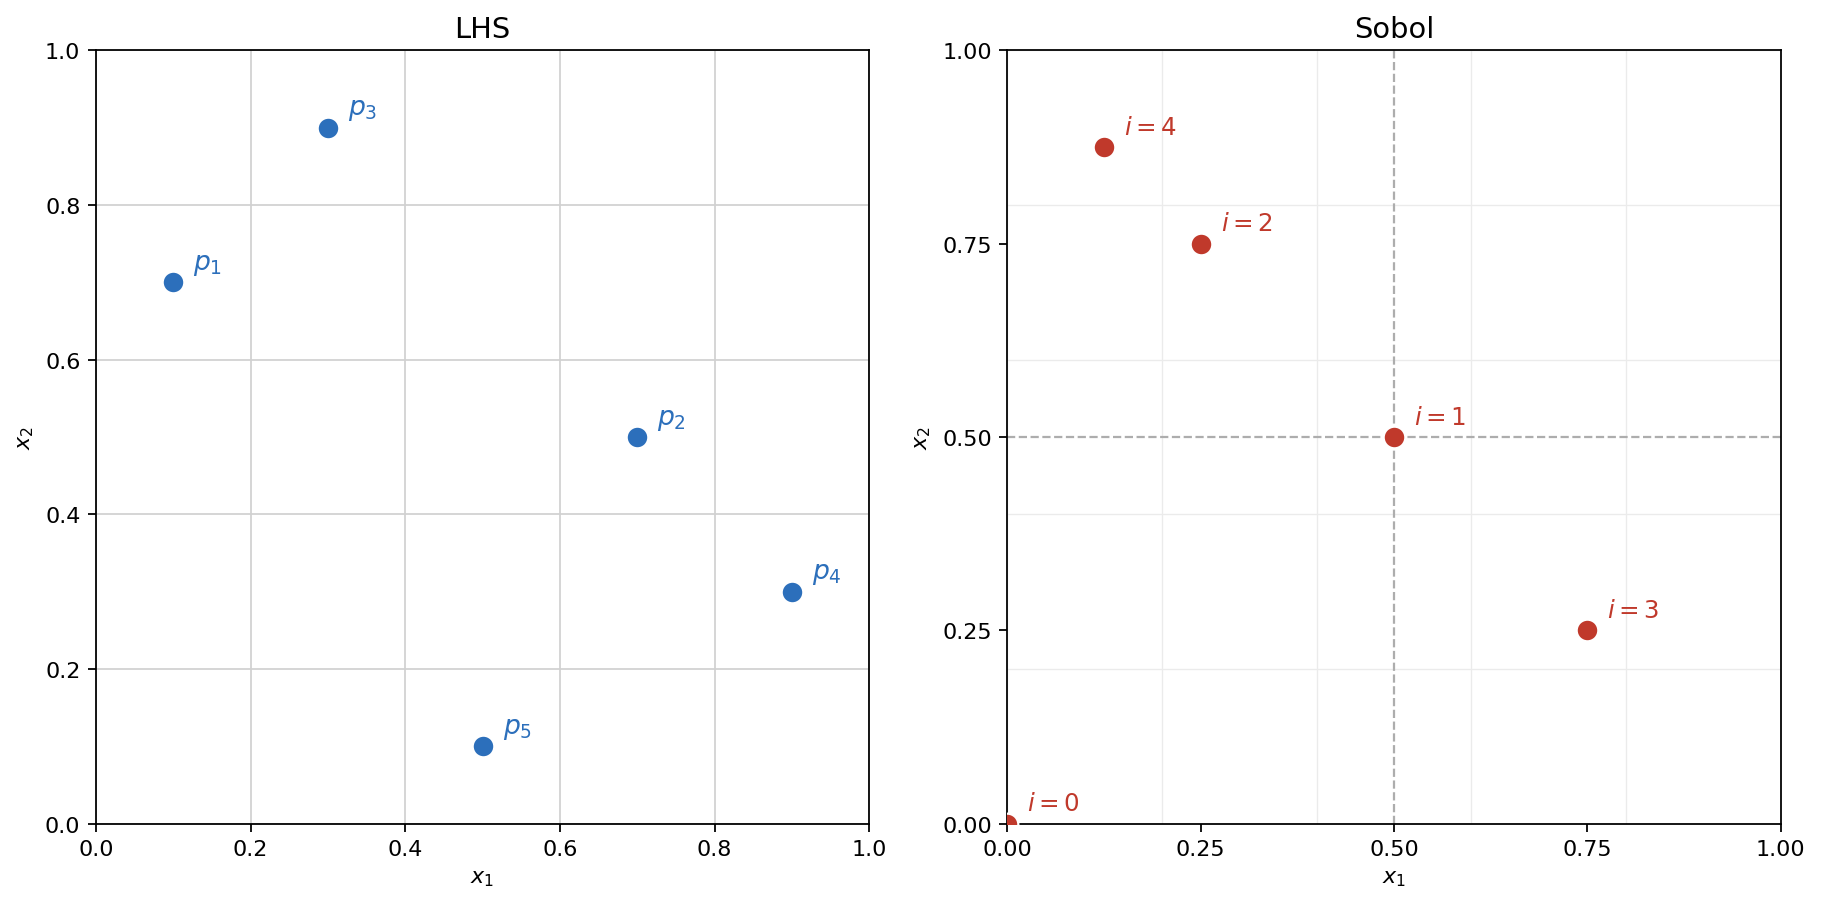
\includegraphics[width=0.9\textwidth]{images/comp_lhs_sobol.png}
    \caption{Comparação entre os cinco pontos amostrais obtidos por LHS (esquerda) e pelos primeiros cinco pontos da sequência de Sobol (direita) no domínio $[0,1]^2$.}
    \label{fig:comp_lhs_sobol}
\end{figure}

A distinção prática entre as duas técnicas aparece quando se observa a distribuição conjunta das amostras. O LHS garante que cada faixa unidimensional seja preenchida uma única vez, mas não exerce controle sobre o espaçamento dos pontos quando as dimensões são consideradas em conjunto, o que pode deixar agrupamentos ou vazios no interior do domínio, limitação que motiva variantes como o maximin discutido anteriormente. O Sobol, por construção, busca a uniformidade também nas projeções de dimensão superior, o que tende a produzir um preenchimento mais regular. Essa vantagem se acentua à medida que o número de dimensões cresce, motivo pelo qual o Sobol costuma ser preferido em problemas com muitos parâmetros de entrada. 
Analisando a Figura \ref{fig:comp_lhs_sobol}, nota-se que a distribuição de Sobol preenche o espaço de forma mais sitemática e entende-se que os espaços vazios deixados são consequência do número reduzido de pontos amostrais. Por outro lado, a abordagem por LHS gera um conjunto no qual os espaços vazios são consequência da estocasticidade associada à permutação realizada durante seu cálculo.

Retomando a questão levantada ao final da apresentação do LHS, ambas as construções descritas até aqui pressupõem que cada parâmetro varia livremente dentro do seu intervalo, de forma independente dos demais. Essa hipótese é adequada quando se amostram hiperparâmetros soltos, mas deixa de valer no caso de uma carteira de ativos. Ao tratar os pesos $w_i$ como coordenadas do espaço amostral, surge a restrição $\sum_i w_i = 1$. Um ponto gerado diretamente por LHS ou Sobol no cubo $[0,1]^d$ dificilmente satisfaz essa igualdade, de modo que a amostragem no cubo, tomada isoladamente, não produz carteiras válidas. A amostragem, portanto, não deve recair sobre um cubo livre e sim sobre uma figura geométrica denominda simplex, definida formalmente como:
\begin{equation}
\Delta^{n-1} = \Big\{ \mathbf{w} \in \mathbb{R}^n : w_i \geq 0, \ \textstyle\sum_{i=1}^{n} w_i = 1 \Big\}.
\end{equation}

Para tornar o efeito dessa restrição mais concreto em multiplas dimensões, convém passar ao caso de três ativos, com $d=3$ e pesos $w_1$, $w_2$ e $w_3$. O conjunto dos pontos que satisfazem simultaneamente $w_i \geq 0$ e $w_1 + w_2 + w_3 = 1$ não é o cubo $[0,1]^3$, mas apenas a fatia contida no plano definido por essa igualdade. Essa fatia é um triângulo (um simplex para o caso com $n=3$ dimensões) cujos vértices são $(1,0,0)$, $(0,1,0)$ e $(0,0,1)$, isto é, as três carteiras que concentram todo o capital em um único ativo. Qualquer carteira admissível de três ativos corresponde a um ponto sobre esse triângulo, e o problema de amostragem passa a ser o de distribuir pontos de maneira uniforme sobre ele, e não sobre o volume do cubo.

A Figura~\ref{fig:simplex} ilustra o simplex imerso no espaço tridimensional, com os pontos amostrais restritos ao plano $w_1 + w_2 + w_3 = 1$. Observa-se que, embora o espaço de partida seja o cubo unitário, o conjunto de carteiras válidas ocupa somente a superfície triangular que o atravessa, o que reduz a dimensionalidade efetiva do problema de três para dois graus de liberdade.

\begin{figure}[htbp]
    \centering
    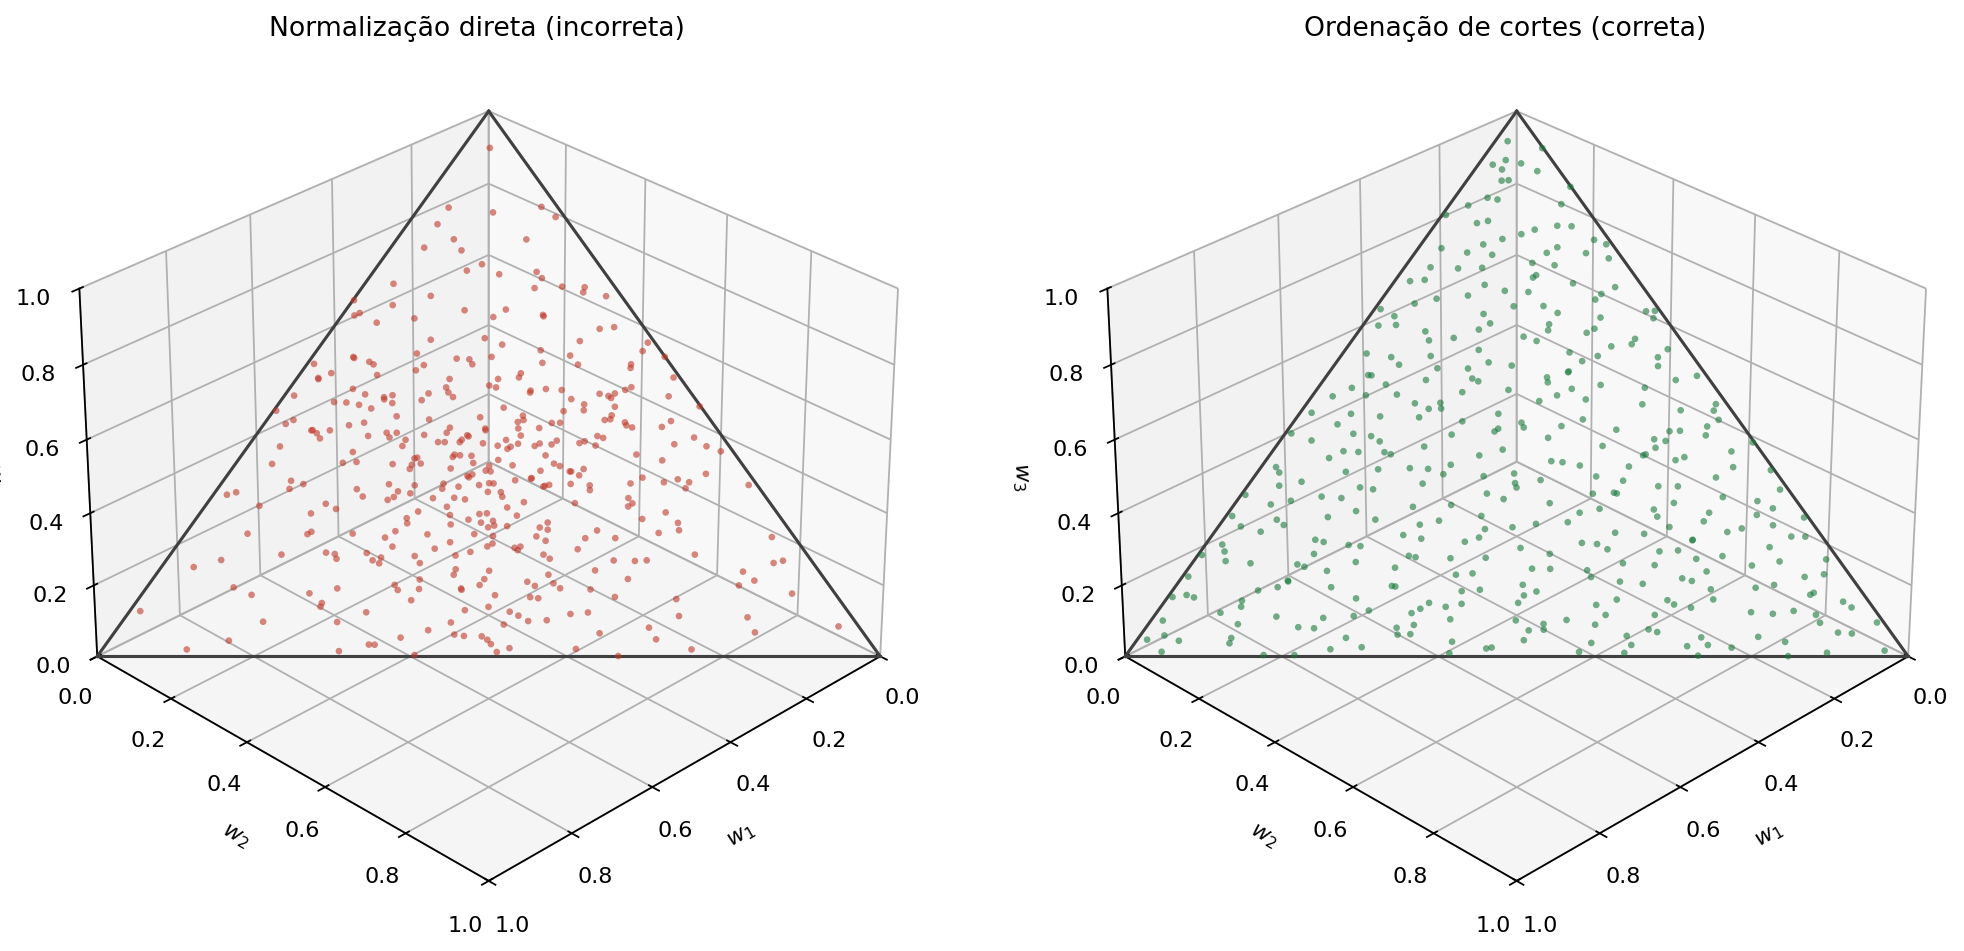
\includegraphics[width=0.95\textwidth]{images/simplex_compare.png}
    \caption{Amostragem sobre o simplex $w_1 + w_2 + w_3 = 1$ com $w_i \geq 0$. À esquerda, a normalização direta dos pontos do cubo concentra as amostras no centro do triângulo; à direita, a ordenação de cortes distribui as amostras de forma uniforme sobre toda a superfície.}
    \label{fig:simplex}
\end{figure}

O modo como se leva uma amostragem do cubo para o simplex determina se a distribuição resultante é adequada ou enviesada. A abordagem imediata consiste em gerar os pontos por LHS ou Sobol no cubo e, em seguida, dividir cada vetor pela soma de suas coordenadas, forçando o resultado a somar um. Esse procedimento, ainda que satisfaça a restrição, não preserva a uniformidade: como a soma de coordenadas aproximadamente uniformes tende a se concentrar em torno de um valor central, a divisão empurra os pontos para o interior do triângulo, deixando as bordas e os vértices pouco representados. No contexto de portfólio, isso significaria testar quase sempre carteiras equilibradas e raramente carteiras concentradas em um ou dois ativos.

Uma forma melhor de mapear as amostras para o simplex preservando a boa distribuição herdada do LHS ou do Sobol é utilizar os resultados das amostragens em $n-1$ dimensões (redução de uma dimensão devido à restrição do simplex) obtidas por esses métodos para posteriormente utilizá-las como cortes ordenados de um intervalo unitário. Ou seja, interpreta-se cada ponto amostrado no domínio $[0,1]^{n-1}$ como um conjunto de $n-1$ cortes sobre o um segmento de reta representativo do intervalo unitário. Assim, ordenando esses cortes e tomando as diferenças consecutivas, obtêm-se $n$ comprimentos que constituem os pesos amostrados. Dessa forma, para $n=3$, a partir de dois valores ordenados $u_{(1)} \leq u_{(2)}$:
$$ w_1 = u_{(1)}, \qquad w_2 = u_{(2)} - u_{(1)}, \qquad w_3 = 1 - u_{(2)} $$
Por construção, os pesos são não negativos e somam um, sem rejeição de pontos nem normalização por soma. Como a operação de ordenar e diferenciar é suave, o espalhamento dos cortes se traduz diretamente no espalhamento dos pesos, preservando a cobertura do amostrador de origem. A Figura~\ref{fig:simplex} contrasta as duas abordagens: no painel da esquerda, a normalização direta concentra as amostras no centro do triângulo; no painel da direita, a ordenação de cortes cobre o simplex de maneira uniforme. Dessa forma, é possível conciliar as propriedades desejáveis das sequências amostrais com a restrição estrutural imposta pela composição de uma carteira, garantindo que a superfície aproximada da função objetivo seja construída sobre um conjunto de carteiras representativo de todo o espaço admissível.





\subsection{Modelos substitutos e otimização bayesiana}
\label{sub:surrogate}

Cada carteira possível pode ser vista como um ponto de um mapa cuja altura representa o seu desempenho, por exemplo o Sharpe da carteira. O objetivo é achar o pico mais alto. A dificuldade é que não se enxerga o terreno inteiro: para conhecer a altura em um ponto é preciso medir, e cada medição é cara, pois envolve simular o desempenho da carteira sob incerteza. Com orçamento de medições limitado, a pergunta é como achar o pico gastando o mínimo de avaliações. Essa é exatamente a pergunta da otimização bayesiana.

Em vez de medir o terreno todo, fazem-se algumas medições espalhadas e, a partir delas, constrói-se um palpite educado sobre a superfície inteira, inclusive onde não se mediu. Esse palpite barato de consultar é o modelo substituto. O substituto mais usado é o processo gaussiano \cite{rasmussen2006gaussian}, que fornece, para cada ponto $\mathbf{w}$, não apenas uma média prevista $\hat{\mu}(\mathbf{w})$, mas também uma medida de incerteza $\hat{\sigma}(\mathbf{w})$ sobre essa previsão. Perto de onde se mediu, a incerteza é pequena, enquanto longe do ponto de medição ela é grande. É essa informação de incerteza que orienta onde vale a pena medir em seguida.

A escolha do próximo ponto cabe à função de aquisição, que combina a média prevista e a incerteza para pontuar cada candidato, equilibrando uma tensão entre a explotação e a exploração. A explotação consiste em medir onde o substituto prevê altura alta, apostando no que já parece bom. A exploração consiste em medir onde o substituto está muito incerto, investigando o desconhecido, pois pode haver um pico escondido. Apenas explotar prende a busca em um ótimo local; apenas explorar desperdiça medições em regiões ruins. Esse compromisso é o tema central de \citeonline{moran2026balancing} e reaparece em \citeonline{millar2025bayesian} e \citeonline{you2025improving}.

Uma função de aquisição clássica é a melhoria esperada, ou \textit{Expected Improvement}, de \citeonline{jones1998efficient}. Sendo $f^\ast$ o melhor valor de desempenho encontrado até então, e definindo a melhoria em um ponto como $I(\mathbf{w}) = \max\!\big(f(\mathbf{w}) - f^\ast, 0\big)$, a melhoria esperada sob o processo gaussiano tem forma fechada:
\begin{equation}
\mathrm{EI}(\mathbf{w}) = \big(\hat{\mu}(\mathbf{w}) - f^\ast\big)\,\Phi(z) + \hat{\sigma}(\mathbf{w})\,\phi(z),
\qquad
z = \frac{\hat{\mu}(\mathbf{w}) - f^\ast}{\hat{\sigma}(\mathbf{w})},
\label{eq:ei}
\end{equation}
onde $\Phi$ e $\phi$ são a função de distribuição acumulada e a densidade da normal padrão. O primeiro termo da Equação~\eqref{eq:ei} privilegia a explotação, favorecendo pontos de média alta; o segundo privilegia a exploração, favorecendo pontos de alta incerteza. O ponto de maior EI é o próximo a ser medido.

Sobre a escolha do substituto, cabe notar que o processo gaussiano é o padrão na literatura justamente por fornecer a incerteza de forma natural e bem fundamentada, o que é essencial para a função de aquisição. Modelos da família de árvores, como florestas aleatórias e algoritmos de reforço de gradiente, não fornecem essa incerteza de forma imediata. \citeonline{you2025improving} recorrem a um estimador de estrutura em árvore, o TPE, que constrói a incerteza de outra maneira e escala melhor que o processo gaussiano sob orçamento apertado. Testar tais alternativas é uma linha legítima, condicionada à capacidade de o substituto entregar incerteza utilizável pela função de aquisição.

\subsection{Considerações parciais da revisão}

...

% ===============================================================
%  3. PLANO DE PROJETO
% ===============================================================
\section{Plano de Projeto}
\label{sec:plano}

\subsection{Resumo da abordagem}

...

\subsection{Requisitos do pipeline}

...

\subsection{Formulação do problema de otimização}
\label{sub:formulacao}
...

\subsubsection{Função objetivo}
...

\subsubsection{Retorno e risco}
...

\subsection{Dados}
...

\subsubsection{Ativos no portfólio}
...

\subsubsection{Coleta e pré-processamento}
O histórico de preços é obtido pela API da Yahoo Finance, de acesso simples e gratuito, o que viabiliza o projeto dentro das restrições de tempo e recurso. Trabalha-se com uma lista pré-definida de ações conhecidas da bolsa americana, de fácil acesso pela API. Evitam-se empresas que faliram no período, atento ao viés de sobrevivência. Por transparência metodológica, vale ressaltar que a expectativa é de que a escolha das ações tenha efeito desprezível sobre o processo de otimização em si, cujo funcionamento independe de quais ativos específicos compõem a lista.

Adotam-se dados diários, pela maior granularidade e para evitar o problema de dispor de poucos pontos de observação. Utiliza-se o preço ajustado, e não o preço bruto, porque o ajuste corrige eventos como pagamento de dividendos e desdobramentos, evitando saltos artificiais que o modelo confundiria com risco real.


\subsection{Metamodelagem}
...

\subsubsection{Projeto de experimentos (DoE)}

Um único ponto não basta para treinar o substituto, ele precisa de várias carteiras espalhadas para começar a enxergar o formato da superfície. O projeto de experimentos é, por isso, a primeira etapa da busca, e a qualidade dessa amostragem inicial condiciona diretamente a qualidade do substituto. Gera-se um conjunto inicial de carteiras por LHS ou por sequências de Sobol, respeitando a geometria do simplex, conforme discutido na revisão, para preservar as propriedades de cobertura. Cada carteira desse conjunto é avaliada pela camada financeira, e com esses pares carteira-desempenho constrói-se o primeiro modelo substituto. A utilização de LHS ou sequências de Sobol depende da dimensão da carteira analisada, dado que a eficiência de cada método depende desse fator.

\subsubsection{Metamodelos}
...

\subsubsection{Exploração e explotação}
...

\subsection{Métodos avaliativos}
...

\subsubsection{Critério de parada}
...
\subsubsection{Validação}
...
\subsubsection{Visualização}
...

% ===============================================================
%  REFERÊNCIAS
% ===============================================================
\newpage
\bibliography{refs}

\end{document}